%% Kevin Depue & Lucas Ellis (2006)
%% opCPP Manual

%% DOCUMENT CLASS
\documentclass[12pt,letterpaper,oneside,fancyhdr]{book}

%% PACKAGES
\usepackage[english]{babel}
\usepackage{geometry}
\geometry{verbose,top=0.5in,bottom=0.5in,letterpaper,lmargin=1in,rmargin=1in}
\usepackage{graphicx}
\usepackage{url}
\usepackage{fix-cm}
\usepackage{setspace}
\usepackage{opcpp}
\usepackage{fullpage}
\usepackage{hyperref}

%% set the default sans-serif font
\usepackage[T1]{fontenc}
\usepackage[scaled]{berasans}
\renewcommand*\familydefault{\sfdefault}  %% Only if the base font of the document is to be sans serif

%% set the default typewriter font
\usepackage[T1]{fontenc}
\usepackage[scaled]{beramono}
%% \renewcommand*\familydefault{\ttdefault} %% Only if the base font of the document is to be typewriter style

%% COMMANDS
\setlength{\parindent}{0em}

%%DOCUMENT START
\begin{document}

%% TITLE PAGE
\begin{center}
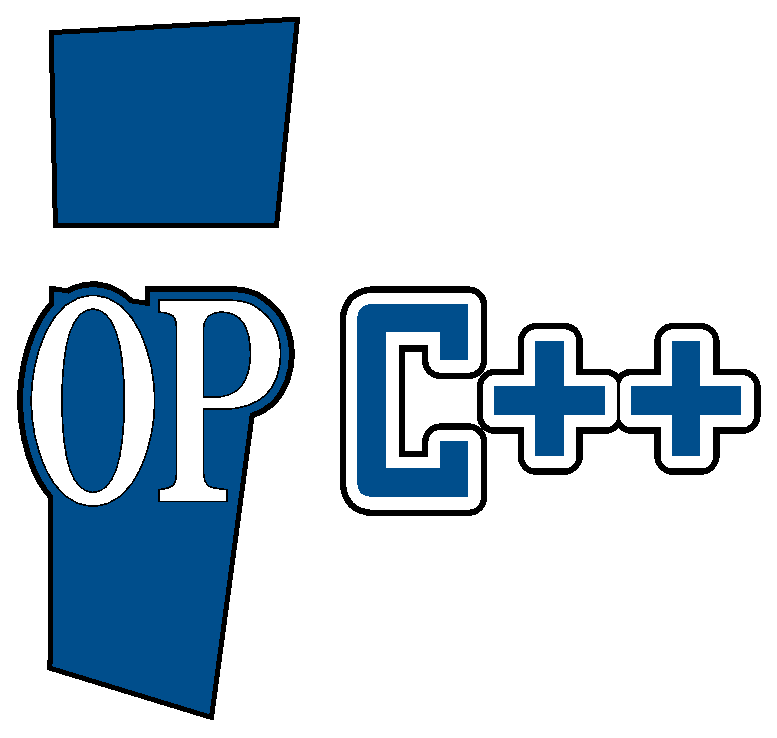
\includegraphics[scale=.9]{opcpp.eps}\\
\vspace{2in}
{\fontsize{50}{60}\selectfont \opCPP\ Manual}\\
\vspace{6mm}
{\Large OP Games LLC \copyright\ 2007}\\ 
\vspace{3mm}
{\Large \url{www.opcpp.com}}
\thispagestyle{empty}
\end{center}
\newpage

%% TABLE OF CONTENTS
\tableofcontents
\clearpage
\pagebreak

%% INTRODUCTION
%% ************
%% INTRODUCTION
%% ************

% introduction
\chapter{Introduction}
\label{chap:introduction}

% history
\section{History}

\opCPP\ was originally created as a means to speed up computer game development.  The standard programming language for games is \cpp\ due to its speed.  However, there are several nuances in \cpp\ that can make game programming tedious.  One of the most pronounced is serialization, i.e., the process of mapping class data members to memory.  Writing this kind of code can also be difficult to read.  We set out to write a source to source compiler transforming a new extended version of \cpp\ (\opCPP) to standard \cpp\ code that can then be compiled by an optimizing back-end compiler.  In the process, we added several new features to the language that are extremely useful, but very difficult to emulate in standard \cpp\ manually.  Examples include beautification of several \cpp\ constructs (e.g., macros), full data-mapping support for objects, state support for classes, a powerful new preprocessor that allows you to nest macros to any depth, and several new up and coming features such as interfaces/mixins/trait support.  New features will continue to be added to this language as development progresses.

% overview
\section{Overview}

In this manual we describe the syntax and proper usage of the \opCPP\ language.  Since \opCPP\ is largely a generative programming language, it should be noted that much of the syntax and usage described can be altered.  What is not alterable is the validation of the code performed before the code is translated - which makes this manual very useful even when concrete examples are given.  It should also be mentioned that we have the goal of making our language and compiler \cpp\ friendly.  However, we don't to the extent of making validation not possible.  As a result keep in mind that the syntax is often context dependent, and what works in an \opCPP\ class will not work in a \cpp\ class or have the same implications when compiled with \opCPP.  Another rule of \opCPP\ is for the default setup to have the same overhead and performance as normal \cpp.  You don't need to look out for any hidden costs when using \opCPP, other than the ones you yourself add by hooking in generated code.  The second focus of this manual is on the \opCPP\ compiler.  Topics covered are its proper usage, how you can use it to customize \opCPP, and how to use it to generate code.  The syntax for dialects is also covered in detail in the final chapters.

\clearpage
\pagebreak

%% CONSTRUCTS
%% **********
%% CONSTRUCTS
%% **********

% constructs
\chapter{Constructs}
\label{chap:constructs}

\section{opobjects}
\label{sec:opobject}

opobjects are the object oriented class construct in \opCPP.  They may be defined with a number of keywords, the defaults being \opcppK{opclass} and \opcppK{opstruct}.  Most custom syntax in \opCPP\ is related to opobject contexts.

\subsection{categories}

New types of opobjects may be added by specifying user-defined opobject keywords.  These opobject keywords are called categories.  Categories add additional control for syntax and validation, and can help customize the code generated by the \opCPP\ compiler.   The default categories, \opcppK{opclass} and \opcppK{opstruct}, are in place to provide similar syntax to \cpp, while allowing you to write \opCPP\ and \cpp\ code side by side.

\subsection{{\tt opclass}}

\opcppK{opclass} is the default keyword to start a class-based opobject construct.  The syntax for declaring an\opcppK{opclass} is very similar to the \cpp\ \opcppK{class} construct.  Figure \ref{fig:opclass1} shows a simple \opcppK{opclass} declaration.

% fig:opclass1
\begin{opcpp}[label={fig:opclass1},caption={A simple \opcppK{opclass} declaration in \opCPP.}]
// A simple opclass declaration.
opclass classname
{
	//class definition
};
\end{opcpp}

Inheritance for an \opcppK{opclass} is similar to \cpp\ \opcppK{class} inheritance.  Notable differences are that only single inheritance is currently allowed, and visibility keywords are required and not optional.  Figure \ref{fig:opclass2} makes these differences clear.  The member definitions are also slightly different than in \cpp.  This is covered in Section \ref{}.  Finally, as in \cpp, by default everything is declared \opcppK{private}.

% fig:opclass2
\begin{opcpp}[label={fig:opclass2},caption={Examples of valid and invalid \opcppK{opclass} inheritance.}]
// A valid opclass inherited from parentclass.
opclass classname : public parentclass
{
	// class definition
};

// An invalid opclass - multiple inheritance is not allowed.
opclass classname : public parentclass, public parentclassb
{
	// class definition
}

// An invalid opclass - missing visibility keyword.
opclass classname : parentclass
{
	// class definition
}
\end{opcpp}

\subsection{{\tt opstruct}}

The second default opobject category is \opcppK{opstruct}.  \opcppK{opstruct} is the keyword for \opCPP\ structures.  As an obobject category, the syntax and restrictions match those of \opcppK{opclass} entirely.  The only difference is that, just as in \cpp, its default member visibility is \opcppK{public} instead of \opcppK{private}.  Figure \ref{fig:opstruct1} shows an example of a simple \opcppK{opstruct}.

% fig:opstruct1
\begin{opcpp}[label={fig:opstruct1},caption={A simple \opcppK{opstruct} declaration in \opCPP.}]
// A simple opstruct declaration.
opstruct classname
{
	int a;
	int b;
};

\end{opcpp}

\subsection{user-defined opobjects}

Users may define their own opobject categories.  These simply take the form of additional keywords.  These extra keywords are syntax validated by the compiler, and placement of category keywords in invalid contexts is disallowed.  These options can be enabled via the commandline or through dialects.  See Section \ref{} for instructions on doing this.  Figure \ref{fig:udopobject2} shows an example of a user-defined obobject category.

% fig:udopobject2
\begin{opcpp}[label={fig:udopobject2},caption={A user-defined opobject category declaration called \opcppK{nativeclass}.}]
// A user-defined opoboject category called nativeclass.
nativeclass classname
{
	// class definition
};
\end{opcpp}

\section{{\tt openum}}

In \opCPP, just as we have special keywords for opobjects, we also have a custom syntax for enumerations.  Parsed enumerations are called \opcppK{openum}s, and have the same syntax as \cpp\ \opcppK{enum}s.  Using an \opcppK{openum} instead of a \cpp\ \opcppK{enum} allows \opCPP\ to generate additional code for the enumeration.  Figure \ref{fig:openum1} shows some example \opcppK{openum} declarations.

\begin{opcpp}[label={fig:openum1},caption={Some simple \opcppK{openum} declarations in \opCPP.}]
// A simple Color openum declaration.
// Notice the comma after the entry "Blue" is allowed.
openum Color
{
	Red,
	Blue,
};

// A simple musical genre openum declaration.
// Notice there is no comma after the entry "Country".
openum Genre
{
	Jazz,
	Classical,
	Country
};
\end{opcpp}

\section{{\tt state}}

One special opobject context construct in \opCPP\ is the \opcppK{state}.  This is an alternative to writing switch statements based on the internal state of an object.  The \opcppK{state} construct is used to provide a more descriptive form for state switching code.  Each \opcppK{state} can contain function definitions.  Functions with matching names and signatures will be redirected when called based on the internal state of the object.  In Figure \ref{fig:state1}, calls to the function \opcppK{clicked} will be routed through the internal state.

\begin{opcpp}[label={fig:state1},caption={An example of using the \opcppK{state} construct in \opCPP.}]
// An opclass definition with state support.
opclass ButtonClass
{
	state buttonup
	{
		void clicked()
		{
			// go down
		}	
	}
	
	state buttondown
	{
		void clicked()
		{
			// stay down
		}
	}
};
\end{opcpp}

By default, the internal \opcppK{state} is tracked by a hidden data member, and may be set using the \opcppK{setinternalstate} function.  Figure \ref{fig:state2} shows how to change the \opcppK{state} of the \opcppK{ButtonClass} defined in Figure \ref{fig:state1}.

\begin{opcpp}[label={fig:state2},caption={Changing the internal \opcppK{state} of an instance of \opcppK{ButtonClass} defined in Figure \ref{fig:state1}.}]
ButtonClass b;

b.setinternalstate(ButtonClass::buttonup);
b.clicked();
\end{opcpp}





\clearpage
\pagebreak

%% MODIFIERS
%% *********
%% MODIFIERS
%% *********

% modifiers
\chapter{Modifiers}
\label{chap:modifiers}

Modifiers are new keywords that can appear in front of data members and functions inside {\tt opobject}s (see Section \ref{sec:opobject}).  Modifiers imply that code is generated for them - however by default they do not generate any code on their own.  There are a number of built in modifiers which serve some special purpose - generally they imply special transformations by the compiler.  Modifiers are not a free form type of meta-data like run-time attributes.  Instead, they are strictly checked for correctness and only enabled by dialects.

%% DATA MODIFIERS
\section{Data Modifiers}

Data modifiers are keywords on the front of a data member declaration.  They imply that code should be mapped to a particular variable.  The underlying meaning of modifiers is dependant upon the dialect used.  Multiple modifiers may be applied to a single data member, though applying duplicate modifiers to a single variable results in an error.  The meaning of modifiers may also be dependent upon the opobject category type and dialect.  Figure \ref{fig:datamodifier1} shows an \opcppK{opclass} that uses all of the data modifiers introduced in this section.

% fig:datamodifier1
\begin{opcpp}[label={fig:datamodifier1},caption={An \opcppK{opclass} that uses all the data modifiers introduced in this section.}]
// An opclass with data modifiers.
opclass SomeClass
{
	// Here, x is protected and native.
	protected native int x;

	// Here, y is public and transient.
	public transient int y;

	// Here, z is private, serialized and mapped.
	private int z;
};
\end{opcpp}

\subsection{{\tt native}}

The \opcppK{native} data modifier implies that the data member is not mapped and not serialized.  The exact underlying meaning of mapped and serialized is dependant on the dialect.  Generally, the reason you want a mapped variable is for reflection, while serialized variables are a smaller subset - e.g., writing variables to a file or network stream.  Though declaring a variable \opcppK{native} means that it is not mapped or serialized, you may still link code to \opcppK{native} variables.  You may also disable the \opcppK{native} modifier; this is covered in Section \ref{}.  

\subsection{{\tt transient}}

The \opcppK{transient} data modifier implies that the data member is mapped but not serialized.  You may disable the \opcppK{transient} modifier; this is covered in Section \ref{}.

\subsection{no modifier}

When a data member is declared without a native or transient modifier, it is mapped and serialized.

\subsection{user-defined modifiers}

The real advantage of data modifiers comes from user-defined modifiers.  This makes them similar to attributes in other languages, except the exact context for a modifier must be valid, and they imply behavior at compile time.  The validation aspect of modifiers and modifier combinations will be explored in the future.  The method to enable user defined data modifiers is covered in Section \ref{}.  Figure \ref{fig:datamodifier2} shows some possible user-defined data modifiers within an \opcppK{opclass}.

% fig:datamodifier2
\begin{opcpp}[label={fig:datamodifier2},caption={Some possible user-defined data modifiers.}]
// An opclass definition.
opclass ClassName
{
	// User-defined modifiers (reliable, unreliable,
	// server, client).
	reliable server float health;
	unreliable client string message;
};

// An opstruct definition.
opstruct StructName
{
	// User-defined modifier (compressed).
	float x;
	float y;
	compressed float z; 
}

\end{opcpp}

%% FUNCTION MODIFIERS
\section{Function Modifiers}

Function modifiers are a concept similar to data modifiers.  They are in the form of keywords on the front of member function declarations and definitions.  While not so useful for serialization, they may be useful for instrumenting code or for providing reflection meta-data about functions.

\subsection{{\tt delegate}}

The \opcppK{delegate} modifier is a special modifier handled in \opCPP.  It allows you to generate code for a delegate handler, while linking a default function definition to the handler.  The \opcppK{delegate} modifier is only valid on function definitions, and not prototypes.  Figure \ref{fig:delegate1} shows an example of this.

% fig:delegate1
\begin{opcpp}[label={fig:delegate1},caption={the delegate function modifier in \opCPP.}]
// An opclass definition.
opclass ClassName
{
	// A delegate definition.
	delegate void onclick()
	{
		// do default click stuff
	}
};
\end{opcpp}

\subsection{{\tt inline}, {\tt uninline}}

Function inlining in \opCPP\ is slightly different than in normal \cpp.  In major \cpp\ compilers, member functions declared in headers are inlined by default, or else the \opcppK{inline} keyword can be used to indicate this.  In \opCPP\ you can also \opcppK{uninline} functions, which removes them from the headers and places them in a single source compilation unit.  In \opCPP, the default is to \opcppK{uninline} functions, meaning major compilers will generally not \opcppK{inline} the functions.  The reasoning behind this is that functions should only be inlined when a profiler tells you to - this is common \cpp\ advice to prevent code bloat.  This behavior can be switched back to the \cpp\ defaults while preserving the \opcppK{uninline} keyword via a command-line option.  Figure \ref{fig:inline1} shows an example of using the \opcppK{inline} and \opcppK{uninline} keywords.

% fig:inline1
\begin{opcpp}[label={fig:inline1},caption={Using the \opcppK{inline} and \opcppK{uninline} keywords in \opCPP.}]
// An opclass definition.
opclass ClassName
{
	// An inline function definition.
	inline float squared(float x)
	{
		return x * x;
	}

	// An uninlined function definition.
	uninline float squaredsquared(float x)
	{
		return squared(squared(x));
	}

	// Uninlined by default!
	void function()
	{
		// do stuff
	}
};
\end{opcpp}

\pagebreak

\subsection{{\tt user defined}}

You can also create and use user-defined function modifiers in \opCPP.  While less useful than data modifiers, they can provide instrumentation and reflection for binding other languages to function calls.  Figure \ref{fig:userfunctionmodifiers1} shows a possible user-defined function modifier in \opCPP.

% fig:functionmodifiers1
\begin{opcpp}[label={fig:userfunctionmodifiers1},caption={User-defined function modifiers in \opCPP.}]
// An opclass definition.
opclass ClassName
{
	// Here a user defined modifier is used (event).
	event void incoming(string message);

	// You can mix C++ and opC++ modifiers together.
	static native void outgoing(string message);
};
\end{opcpp}

%% OTHER MODIFIERS
\section{Other Modifiers}

\subsection{{\tt public}, {\tt private}, {\tt protected}}

Some of the most useful modifiers are the visibility modifiers \opcppK{public}, \opcppK{private} and \opcppK{protected}.  These can be applied to both functions and data members in opobjects.  They do the same thing as the normal \cpp\ visibility labels, but only apply to a single member at a time.  They are aware of the default visibility and can be used together with normal \cpp\ visibility labels.  Figure \ref{fig:vismodifiers1} shows an example of this.

% fig:vismodifiers1
\begin{opcpp}[label={fig:vismodifiers1},caption={Visibility modifiers \opcppK{public}, \opcppK{private} and \opcppK{protected} in \opCPP.}]
// An opclass definition.
opclass ClassName
{
private:
	public    int publicmember;
	protected int protectedmember;
	          int privatemember;
};
\end{opcpp}

\clearpage
\pagebreak

%% MACROS
%% ******
%% MACROS
%% ******

% macros
\chapter{Macros}
\label{chap:macros}

\opCPP\ improves the way in which you can write \cpp\ macros.  It also provides a new powerful preprocessor via the \opcppK{opmacro} keyword.

\section{{\tt opdefine}}
\label{sec:opdefine}

\opcppK{opdefine} is a replacement for the \cpp\ \opcppK{#define} statement.  It's syntax is nicer, and it will automatically call \opcppK{#undef} on the symbol to be defined.  Figure \ref{fig:opdefine1} shows an example of a simple \cpp\ macro and the corresponding equivalent in \opCPP.  \opcppK{opdefine} can also be used for macros that have arguments.  Figure \ref{fig:opdefine2} shows an example of this.  \opcppK{opdefine} can have comments within them also, making them much easier to document than \cpp\ \opcppK{#define} statements.

% fig:opdefine1
\begin{opcpp}[label={fig:opdefine1},caption={Simple \cpp\ macro and corresponding equivalent in \opCPP.}]
// A simple C++ macro with undef
#undef SIMPLE
#define SIMPLE void Render();

// The opcpp equivalent.
opdefine SIMPLE
{
	void Render();
}
\end{opcpp}

% fig:opdefine2
\begin{opcpp}[label={fig:opdefine2},caption={\opcppK{opdefine} example with arguments.}]
// A simple C++ macro with arguments.
#undef SAFE_DELETE
#define SAFE_DELETE(p)  \
	if (p)				\
		delete (p);		\
	(p) = NULL;

// The opcpp equivalent.
opdefine SAFE_DELETE(p)
{
	if (p)
		delete (p);
	(p) = NULL;
}
\end{opcpp}

One thing to notice about the \opcppK{opmacro} keyword is that because its body is enclosed inside braces, you cannot use the {\tt \{} or {\tt \}} characters by themselves (without their matching brace) as this makes the code impossible to parse.  This is why standard \cpp\ macros use the line termination character \verb!\! for macros.  To get around this issue, we can use \opcppK{#define} to declare and use a single brace, as shown in Figure \ref{fig:opdefine3}.

% fig:opdefine3
\begin{opcpp}[label={fig:opdefine3},caption={Getting around the \opcppK{opdefine} brace issue.}]
// Declare the left brace as a regular C++ macro.
#define LB {

// The opcpp equivalent.
opdefine LOOP_START
{
	while (bKeepLooping)
	LB
		// ... add code here ...
}
\end{opcpp}

\subsection{{\tt macro}}

In order to use \cpp\ macros and \opcppK{opdefine} macros in opObject code, you must prefix the macro call with the \opcppK{macro} keyword.  This is to help resolve ambiguities when parsing.  For example, Figure \ref{fig:macro1} shows how to call the macros defined in Section \ref{sec:opdefine} in \opCPP.

% fig:macro1
\begin{opcpp}[label={fig:macro1},caption={How to correctly call the macros defined in Section \ref{sec:opdefine} in \opCPP.}]
// Simple macro call.
macro Simple

// SAFE_DELETE macro call.
SomeObject* x = new SomeObject();
macro SAFE_DELETE(x)

// ADD_FUNCTION macro call.
macro ADD_FUNCTION
\end{opcpp}

\pagebreak
\section{{\tt opmacro}}

\opCPP\ introduces a new internal preprocessor and two new keywords: \opcppK{opmacro} and \opcppK{expand}.  \opcppK{opmacro}s are declared with a syntax similar to \opcppK{opdefine}s.  However, unlike \opcppK{opdefine}s, \opcppK{opmacro}s only have an effect in the \opCPP\ compiler.  They may be defined multiple times, with each new declaration replacing the last.  In addition, \opcppK{opmacro}s are matched by signature (the number of arguments in an \opcppK{opmacro}).  \opcppK{opmacro}s may only be declared in the global namespace.  Finally, \opcppK{opmacro}s may contain comments.  Figure \ref{fig:opmacro1} shows a simple \opcppK{opmacro} instantiation.

% opmacro1 figure
\begin{opcpp}[label={fig:opmacro1},caption={A simple \opcppK{opmacro} instantiation.}]
// An opmacro definition.
opmacro build_function(return_type,name,body)
{
	return_type name()
	{
		// Body will be replaced with the body argument passed in.
		body
	}
}
\end{opcpp}

\opcppK{opmacro}s also define a small number of operators, similar to the way the \cpp\ preprocessor works.  These operators are stringize and paste.  The final syntax for these operators is currently undecided, but they will probably be different than the \cpp\ preprocessor operators for clarity.

\subsection{{\tt expand}}

\opcppK{expand} is an operator that allows you to expand \opcppK{opmacro} definitions.  \opcppK{opmacro}s are only useful when referenced by \opcppK{expand} calls.  \opcppK{expand} and \opcppK{opmacro} calls may also be combined to generate \opcppK{opmacro}s from \opcppK{opmacro}s, or \opcppK{opdefine}s from \opcppK{opmacro}s.  \opcppK{expand} calls may be used in any context, and will be verified against available \opcppK{opmacro}s (by name and signature).  \opcppK{expand} calling arguments may be empty, have one or more tokens, and may include line breaks and whitespace.  In addition, \opcppK{expand} calls are more useful than preprocessor definitions in that the expanded code is fully debuggable, and will point back to the original \opcppK{opmacro} definition via \opcppK{#line} redirection!  Figure \ref{fig:expand1} shows how to use \opcppK{expand} to instantiate the \opcppK{build_function} \opcppK{opmacro} defined in Figure \ref{fig:opmacro1}.

% expand1 figure
\begin{opcpp}[label={fig:expand1},caption={Using an \opcppK{expand} call to instantiate the \opcppK{build_function} \opcppK{opmacro} defined in Figure \ref{fig:opmacro1}.}]
/**** Some expand calls. ****/

// This builds a void function called nothing.
expand build_function(void,nothing,/*do nothing*/)

// This builds a float returning function called process, 
// which returns sqrt(20);
expand build_function(float,process,return sqrt(20);)
\end{opcpp}

Advanced uses for \opcppK{opmacro}s involve using them to build or \opcppK{expand} other \opcppK{opmacro}s or \opcppK{opdefine}s.  In such cases, special rules are used to make the expansions useful.  \opcppK{expand} calls within \opcppK{expand} calls are only called before the outer call is expanded.  \opcppK{expand} calls within \opcppK{opmacro}s are only expanded once the outer \opcppK{opmacro} is expanded.  An example of this is shown in Figure \ref{fig:expand2}.

% expand2 figure
\begin{opcpp}[label={fig:expand2},caption={Advanced use of \opcppK{expand} and \opcppK{opmacro} in \opCPP.}]
// Note that the expand calls will not be called 
// until this opmacro is expanded.
opmacro build_macros(category)
{
	expand build_element_macros(category,int)
	expand build_element_macros(category,float)
	expand build_element_macros(category,bool)
}

// The order doesn't matter here as long as the 
// expansion is done after opmacros are declared.
opmacro build_element_macros(category,tag)
{
	// using the paste operator (##)
	opdefine category##_##tag
	{
	}
}

// Expand for opclass.
expand build_macros(opclass)

// Expand for opstruct.
expand build_macros(opstruct)

// These expand calls will generate the following opdefines
// (and in turn preprocessor #defines):
// opclass_int, opclass_float, opclass_bool,
// opstruct_int, opstruct_float, opstruct_bool.
\end{opcpp}

\clearpage
\pagebreak

%% ALTERNATES
%% **********
%% ALTERNATES
%% **********

\chapter{Alternates}
\label{chap:alternates}

\section{{\tt opinclude}}

The \opcppK{opinclude} keyword is similar to the \opcppK{#include} keyword in \cpp, except that it is used to include {\tt .oh} files.  \opCPP\ ignores the \opcppK{#include} command, but if the \opcppK{opinclude} keyword is hit, it will load and parse the file specified.  Figure \ref{fig:opinclude1} shows how to use \opcppK{opinclude}.  \opCPP\ will look for the file to be included in every directory specified on the command line and in the current working directory.

% fig:opinclude1
\begin{opcpp}[label={fig:opinclude1},caption={The \opcppK{opinclude} keyword.}]
opinclude "SomeFile.oh"
\end{opcpp}

\section{{\tt opdefine}}

See Section \ref{sec:opdefine}.

\section{{\tt opstatic}}

The \opcppK{opstatic} keyword is an {\tt opobject}-specific keyword that makes it easier to initialize static class members.  In standard \cpp, you must declare a static variable in the header file and initilize its default value in the source file.  The \opcppK{opstatic} keyword allows you to declare a static variable in the header file and initialize it in place.  Figure \ref{fig:opstatic1} shows an example of this.  Unlike modifiers (see Section \ref{chap:modifiers}), the order of keywords in an \opcppK{opstatic} declaration matters.  The \opcppK{opstatic} keyword must be the first keyword in the declaration - this may be changed in the future.  Figure \ref{fig:opstatic2} makes this clear.  Finally, it is not necessary to set an \opcppK{opstatic} variable to a value.  You can simply declare the variable as \opcppK{opstatic}, as shown in Figure \ref{fig:opstatic3}.

% fig:opstatic1
\begin{opcpp}[label={fig:opstatic1},caption={The \opcppK{opstatic} keyword.}]
/**** The static keyword in normal C++. ****/

// Header file.
class Actor
{
private:
	static bool bRenderable;
};

// Source file.
bool Actor::bRenderable = true;

/**** The opstatic replacement keyword in opC++. ****/ 

// Header file.
opclass Actor
{
private:
	opstatic bool bRenderable = true;
};
\end{opcpp}

% fig:opstatic2
\begin{opcpp}[label={fig:opstatic2},caption={The \opcppK{opstatic} keyword must come first in an \opcppK{opstatic} declaration.}]
// Invalid syntax (opstatic is not the first keyword).
opclass A
{
private:
	public opstatic int x = 3;
};

// Valid syntax (opstatic is the first keyword).
opclass A
{
private:
	opstatic public int x = 3;
};
\end{opcpp}

% fig:opstatic3
\begin{opcpp}[label={fig:opstatic3},caption={Declaring a variable \opcppK{opstatic} without initializing it.}]
// opstatic variable without initialization.
opclass A
{
private:
	opstatic public int x;
};
\end{opcpp}


\clearpage
\pagebreak

%% COMMAND LINE
%% ************
%% COMMAND LINE
%% ************

%% COMMANDS
\newcommand{\cloption}[2]{{\tt #1} \\ \hspace*{4ex} #2 \\}

% command line
\chapter{Commandline}
\label{chap:commandline}

This chapter lists all the available commandline options in the \opCPP\ compiler.  An important thing to note is that if a file or directory includes spaces, it must be in quotes!  Also, separate multiple strings with commas and {\em no spaces}.\\

Example:  {\tt opcpp -oh file1.oh,"file 2.oh" -d dir1,dir2 -opobject uclass,scriptclass}

\section{Commands}

% commandline options
\cloption{-oh <files>}{Input files to be compiled.}

\cloption{-d <directories>}{Input file directories, separated by a comma.}

\cloption{-ohd <directories>}{All .oh files within these directories will be parsed.}

\cloption{-gd <directory>}{Generated files output directory.}

\cloption{-globmode}{Enables \opCPP\ glob mode.}

\cloption{-verbose}{Prints verbose output.}

\cloption{-silent}{Only prints out compiler errors and tree (if enabled).}

\cloption{-fm}{User defined function modifiers.}

\cloption{-dm}{User defined data modifiers.}

\cloption{-vdm}{User defined valued data modifiers.}

\cloption{-opobject}{User defined \opCPP\ object types.  Can only contain alphabetic charcters!}

\cloption{--opobject-remove-defaults}{Removes the default \opCPP\ object type specifiers. (\opcppK{opclass}, \opcppK{opstruct})}

\cloption{-nodebug}{Suppress debug line directives (suppress debugging redirection support).}

\cloption{--opmacro-expansion-depth}{Specifies the maximum opmacro expansion depth.}

\cloption{-altclass}{Specify alternative mappings for class categories (syntax: classprefix=category,...).}

\cloption{-altstruct}{Specify alternative mappings for struct categories (syntax: structprefix=category,...).}


\clearpage
\pagebreak

%% BIBLIOGRAPHY
\addcontentsline{toc}{chapter}{References}

\bibliographystyle{plain}
\bibliography{manual}

\end{document}
